In \secref{prior_perturbations} we considered a multiplicative perturbations
of the form \eqref{phi_perturbation} with the $\norminf{\cdot}$ norm.  In
this section we consider other norms, illustrating that other choices
have problems with KL divergence.

\begin{defn}\deflabel{diffable_classes}
    (\citep[Definition 4.5]{zeidler:2013:functional})
%
Let $B_1$ and $B_2$ denote Banach spaces, and let $\ball_1 \subseteq B_1$ define
an open neighborhood of $\phi_0 \in B_1$.  Fix a function $f: \ball_1
\mapsto B_2$.

The function $f$ is {\em directionally differentiable} (also known as a
Gateaux differentiable) if, for any $\phi$ with $\norm{\phi - \phi_0} = 1$,
there exists a linear functional $f^{\mathrm{lin}}: B_1 \mapsto B_2$ such that
%
\begin{align*}
%
\lim_{t \rightarrow 0}
    \frac{f(\phi) - f(\phi_0) -
          f^{\mathrm{lin}}(t (\phi - \phi_0) )
         }{t} \rightarrow 0.
%
\end{align*}
%

Similarly, the function $f$ is {\em boundedly differentiable} (also known as Fr{\'echet} differentiable) at $\phi_0$ if there exists a linear
operator, $f^{\mathrm{lin}}$, such that
%
\begin{align*}
%
\lim_{t \rightarrow 0}
    \sup_{\phi: \norm{\phi - \phi_0} = 1}
    \frac{f(\phi) - f(\phi_0) -
          f^{\mathrm{lin}}(t (\phi - \phi_0))
         }{t} \rightarrow 0.
%
\end{align*}
%
\end{defn}

The

We begin with an example from \citet{averbukh:1967:theory}.

%%%%%%%%%%%%%%%%%%%%%%%%%%%%%%%%%%%%%%%%%%%%%%%%%%%%%%%%%%%%%%%%%%%%%%%%%
%%%%%%%%%%%%%%%%%%%%%%%%%%%%%%%%%%%%%%%%%%%%%%%%%%%%%%%%%%%%%%%%%%%%%%%%%
\begin{ex}\exlabel{averbukh}
%
(\citet[Example 1.9]{averbukh:1967:theory})
%
Consider $(x_1, x_2) \in \mathbb{R}^2$ and the polar coordinates $r :=
\sqrt{x_1^2 + x_2^2}$ and $\theta := \arctan(x_2 / x_1)$.  Let $\{\pi k: k \in
\mathbb{Z} \}$ denote integer multiples of $\pi$.  Define
%
\begin{align*}
%
f(r, \theta) := \begin{cases}
\frac{r^2}{| \sin \theta |} \exp\left( -\frac{r}{|\sin \theta|}\right)
    & \textrm{when } \theta \notin \{\pi k: k \in \mathbb{Z} \} \\
0. & \textrm{when } \theta \in \{\pi k: k \in \mathbb{Z} \}
%
\end{cases}
%
\end{align*}
%
Then $f$ is continuous at $(0, 0)$ and has a directional derivative in every
direction, but is not Fr{\'e}chet differentiable.
%
\begin{proof}
%
It is easy to show that $\sup_{y \ge 0} y \exp(-y) = \exp(-1)$, which is
achieved at $y=1$. So, for any $(r_1, \theta_1)$ and $(r_2, \theta_2)$,
$\abs{f(r_1, \theta_1) - f(r_2, \theta_2)} \le \abs{r_1 - r_2} \exp(-1)$, from
which it follows that $f(r, \theta)$ is continuous at $0$.  Moreover, for any
fixed direction $\theta$, $\fracat{\partial f(r, \theta)}{\partial r}{r=0} = 0$,
so the linear approximation to $f(r, \theta)$ at $(0, 0)$ in any direction is
identically zero.  For any $r > 0$, the error in the linear approximation is
given by $\sup_{\theta} \abs{f(r, \theta) - 0} = r \exp(-1)$, which is achieved
by setting $r / |\sin \theta| = 1$.  Thus the error in the linear approximation
is of order $r$, not smaller.
%
\end{proof}
%
\end{ex}
%%%%%%%%%%%%%%%%%%%%%%%%%%%%%%%%%%%%%%%%%%%%%%%%%%%%%%%%%%%%%%%%%%%%%%%%%
%
See \figref{averbukh_plot} for a plot of \exref{averbukh}.  The function
$f(r, \theta)$ is sufficiently flat in neighborhood of $0$ that its
%
%%%%%%%%%%%%%%%%%%%%%%%%%%%%%%%%%%%%%%%%%%%%%%%%%%%%%%%%%%%%%%%%%%%%%%%%%
%%%%%%%%%%%%%%%%%%%%%%%%%%%%%%%%%%%%%%%%%%%%%%%%%%%%%%%%%%%%%%%%%%%%%%%%%
\begin{figure}[h!]

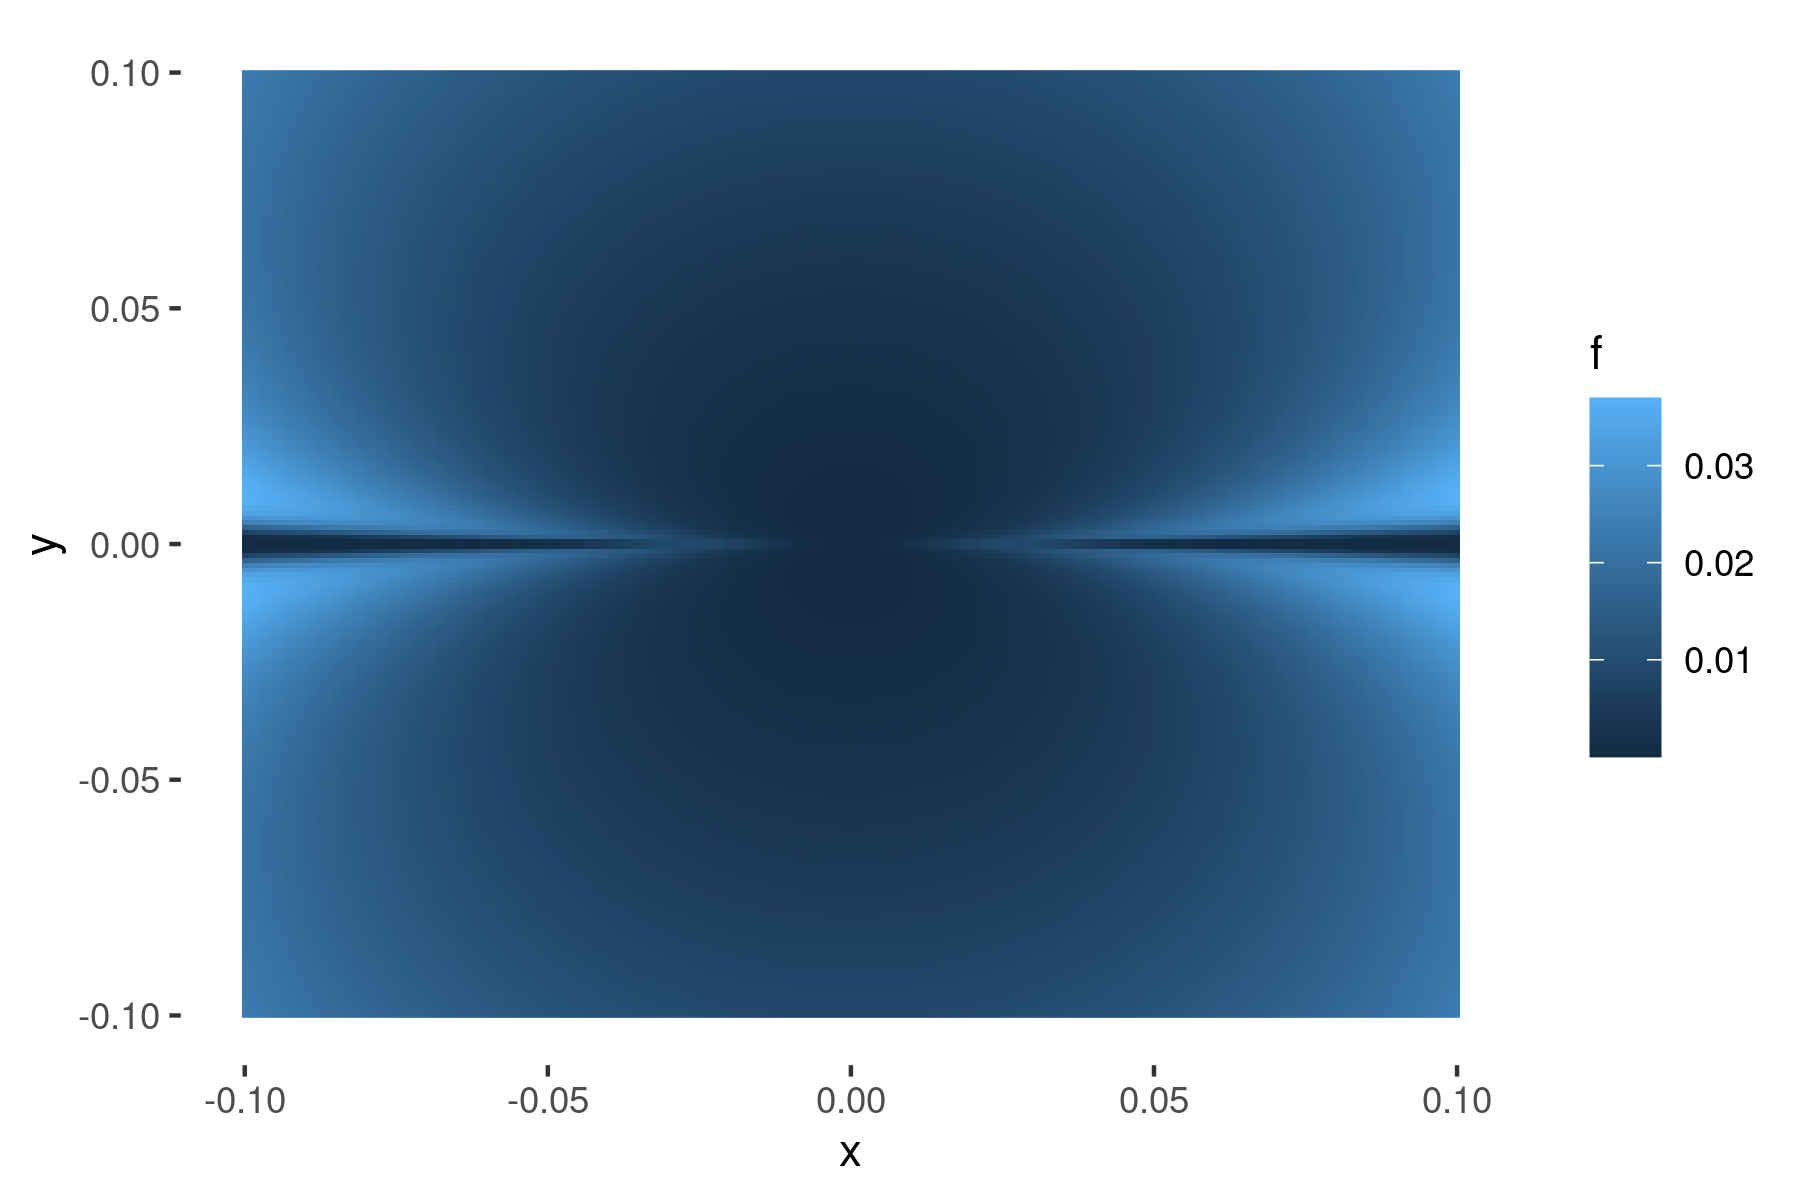
\includegraphics[width=0.980\linewidth,height=0.667\linewidth]{static_images/averbukh_example.png}
\caption{A plot of $f(x_1, x_2)$ from \exref{averbukh}.}\figlabel{averbukh_plot}
\centering
\end{figure}
%%%%%%%%%%%%%%%%%%%%%%%%%%%%%%%%%%%%%%%%%%%%%%%%%%%%%%%%%%%%%%%%%%%%%%%%%
